\documentclass[twocolumn,fleqn,a4paper,10pt]{jarticle}
\usepackage{amsmath,amssymb}
\usepackage[dvipdfmx]{graphicx}
\usepackage{emathT}

\title{微分積分II春課題} 
\date{\today} 

\hoffset = -40pt
\voffset = -110pt
\textwidth = 180mm
\textheight = 275mm

\begin{document}
\setlength{\parindent}{0pt}
\setlength{\columnseprule}{0.4pt}
\setlength{\mathindent}{0pt}

\renewcommand{\thesection}{\fbox{\arabic{section}}}
\renewcommand{\labelenumi}{(\theenumi)}

\maketitle

%1
\section{}
\begin{enumerate}
\item \begin{flalign*}
	&\lim_{x \to -1}\frac{x^2+3x+2}{x^3+x^2+3x+3}\\
	&=\lim_{x \to -1}\frac{(x+2)(x+1)}{(x+1)(x^2+3)}\\
	&=\lim_{x \to -1}\frac{x+2}{x^2+3}\\
	&=\frac{1}{4}
\end{flalign*}
\item \begin{flalign*}
	&\lim_{x \to \infty}\frac{2x^2+9x-5}{3x^2-x-2}\\
	&=\lim_{x \to \infty}\frac{2+\frac{9}{x}-\frac{5}{x^2}}{3-\frac{1}{x}-\frac{2}{x^2}}\\
	&=\frac{2+0-0}{3-0-0}=\frac{2}{3}
\end{flalign*}
\item \begin{flalign*}
	&\lim_{x \to \infty}\frac{1-3^x}{3^{x+1}+2^x}\\
	&=\lim_{x \to \infty}\frac{3^{-x}-1}{3+\frac{2^x}{3^x}}\\
	&=\frac{0-1}{3+0}=-\frac{1}{3}
\end{flalign*}
\item \begin{flalign*}
	&\lim_{x \to 3-0}\frac{|x-3|}{x^2-x+6}\\
	&=\lim_{x \to 3-0}\frac{1}{-x-2}\\
	&=-\frac{1}{5}
\end{flalign*}
\item \begin{flalign*}
	&\lim_{x \to 0}\frac{\sin{5x}}{4x}\\
	&=\lim_{x \to 0}(\frac{\sin{5x}}{5x}\frac{5x}{4x})\\
	&=1\cdot \frac{5}{4}=\frac{5}{4}
\end{flalign*}
\item \begin{flalign*}
	&\lim_{x \to 0}\frac{1-\cos{x}}{x^2}\\
	&=\lim_{x \to 0}\frac{\sin{x^2}}{x^2(1+\cos{x})}\\
	&=\lim_{x \to 0}\frac{\sin{x}}{x}\lim_{x \to 0}\frac{\sin{x}}{x}\lim_{x \to 0}\frac{1}{1+\cos{x}}\\
	&=1 \cdot 1 \cdot \frac{1}{2} = \frac{1}{2}
\end{flalign*}
\item \begin{flalign*}
	&\lim_{x \to 2}\frac{x-2}{\sqrt{x^2+1}-\sqrt{5}}\\
	&=\lim_{x \to 2}\frac{(x-2)(\sqrt{x^2+1}+\sqrt{5})}{x^2-4}\\
	&=\lim_{x \to 2}\frac{\sqrt{x^2+1}+\sqrt{5}}{x+2}\\
	&=\frac{2\sqrt{5}}{4}=\frac{\sqrt{5}}{4}	
\end{flalign*}
\item \begin{flalign*}
	&\lim_{h \to 0}(1+3h)^{\frac{1}{h}}\\
	&=\lim_{h \to 0}(1+3h)^{\frac{3}{3h}}\\
	&=e^3
\end{flalign*}
\end{enumerate}

%2
\section{}
\begin{flalign*}
	\text{(証明)}
	f(x)=x+\log_2{(x^2+1)}-1=0\text{とすると,}\\
	f(x)\text{は}(-\infty.\infty)\text{で連続であり}\\
	f(0)=\log_2{1}-1=-1<0\\
	 f(1)=1+\log_2{2}-1=1>0\\
	\text{よって中間値の定理より}\\
	f(x)\text{は、0と1の間に少なくとも1つの実数解を持つ}\\
	Q.E.D.
\end{flalign*}

%3
\section{}
 \begin{flalign*}
	&f(x)=\sqrt{x}\\
	f'(x)&=\lim_{h \to 0}\frac{f(x+h)-f(x)}{h}\\
	&=\lim_{h \to 0}\frac{\sqrt{x+h}-\sqrt{x}}{h}\\
	&=\lim_{h \to 0}\frac{x+h-x}{h(\sqrt{x+h}+\sqrt{x}}\\
	&=\lim_{h \to 0}\frac{1}{\sqrt{x+h}+\sqrt{x}}\\
	&=\frac{1}{2\sqrt{x}}
\end{flalign*}

%4
\section{}
\begin{enumerate}
\item \begin{flalign*}
	y&=(5x-3)^7\\
	y'&=35(5x-3)^6
\end{flalign*}
\item \begin{flalign*}
	y&=\sqrt{6x+5}\\
	y'&=\frac{3}{\sqrt{6x+5}}
\end{flalign*}
\item \begin{flalign*}
	y&=\frac{4x-3}{x+2}\\
	y'&=\frac{4(x+2)-4x+3}{(x+2)^2}\\
	&=\frac{11}{(x+2)^2}
\end{flalign*}
\item \begin{flalign*}
	y&=\frac{1}{3x^2-1}\\
	y'&=-\frac{6x}{(3x^2-1)^2}
\end{flalign*}
\item \begin{flalign*}
	y&=(x^2+1)^8\\
	y'&=16x(x^2+1)^7
\end{flalign*}
\item \begin{flalign*}
	y&=\frac{10}{3}\sqrt[5]{x^3}\\
	y'&=\frac{10}{3} \frac{3}{5}\frac{1}{\sqrt[5]{x^2}}\\
	&=\frac{2}{\sqrt[5]{x^2}}
\end{flalign*}
\item \begin{flalign*}
	y&=\sqrt[4]{(2x^2+4x+3)^3}\\
	y'&=\frac{3}{4}(2x^2+4x+3)^{-\frac{1}{4}}(4x+4)\\
	&=\frac{3(x+1)}{\sqrt[4]{2x^2+4x+3}}
\end{flalign*}
\item \begin{flalign*}	
	y&=\frac{x}{(1-x)^2}\\
	y'&=\frac{(1-x)^2+2x(1-x)}{(1-x)^4}\\
	&=\frac{1+x}{(1-x)^3}
\end{flalign*}
\item \begin{flalign*}
	y&=(x+1)\sqrt{2x-1}\\
	y'&=\sqrt{2x-1}+\frac{x+1}{\sqrt{2x-1}}\\
	&=\frac{3x}{\sqrt{2x-1}}
\end{flalign*}
\end{enumerate}

%5
\section{}
\begin{enumerate}
\item \begin{flalign*}
	y&=\cos{\frac{x}{4}}\\
	y'&=-\frac{1}{4}\sin{\frac{x}{4}}
\end{flalign*}
\item \begin{flalign*}
	y&=\sin^4{x}\\
	y'&=4\sin^3{x}\cos{x}
\end{flalign*}
\item \begin{flalign*}
	y&=\cos^3{5x}\\
	y'&=-15\cos^2{5x}\sin{5x}
\end{flalign*}
\item \begin{flalign*}
	y&=x^2\cos{\frac{1}{x}}\\
	y'&=2x\cos{\frac{1}{x}}+x^2\sin{\frac{1}{x}}\frac{1}{x^2}\\
	&=2x\cos{\frac{1}{x}}+\sin{\frac{1}{x}}
\end{flalign*}
\item \begin{flalign*}
	y&=\frac{\cos{x}}{1-\sin{x}}\\
	y'&=\frac{-\sin{x}(1-\sin{x})+cos^2{x}}{(1-\sin{x})^2}\\
	&=\frac{-\sin{x}+\sin^2{x}+cos^2{x}}{(1-\sin{x})^2}\\
	&=\frac{1}{1-\sin{x}}
\end{flalign*}
\item \begin{flalign*}
	y&=\sin^2{\frac{1}{\sqrt{x}}}\\
	y'&=2\sin{\frac{1}{\sqrt{x}}}\cos{\frac{1}{\sqrt{x}}}(-\frac{1}{2x\sqrt{x}})\\
	&=-\frac{1}{x\sqrt{x}}\sin{\frac{1}{\sqrt{x}}}\cos{\frac{1}{\sqrt{x}}}\\
\end{flalign*}
\item \begin{flalign*}
	y&=x^2\tan{x}\\
	y'&=2x\tan{x}+x^2\sec^2{x}\\
	&=x(2\tan{x}+x\sec^2{x})
\end{flalign*}
\item \begin{flalign*}
	y&=\frac{1+\tan{x}}{1-\tan{x}}\\
	y'&=\frac{\sec^2{x}(1-\tan{x})+\sec^2{x}(1+\tan{x})}{(1-\tan{x})^2}\\
	&=\frac{2\sec^2{x}}{(1-\tan{x})^2}
\end{flalign*}
\item \begin{flalign*}
	y&=\arcsin{\frac{x}{2}}\\
	y'&=\frac{\frac{1}{2}}{\sqrt{1-\frac{x^2}{4}}}\\
	&=\frac{1}{\sqrt{4-x^2}}
\end{flalign*}
\item \begin{flalign*}
	y&=\arctan{\frac{2}{x}}\\
	y'&=\frac{-\frac{2}{x^2}}{1+\frac{4}{x^2}}\\
	&=-\frac{2}{x^2+4}	
\end{flalign*}
\item \begin{flalign*}
	y&=\log{(x^2+3x+1)}\\
	y'&=\frac{2x+3}{x^2+3x+1}
\end{flalign*}
\item \begin{flalign*}
	y&=\log{\left|\frac{1+x}{1-x}\right|}\\
	y'&=\frac{\frac{1-x+1+x}{(1-x)^2}}{\frac{1+x}{1-x}}\\
	&=\frac{2}{1-x^2}
\end{flalign*}
\item \begin{flalign*}
	x&=(e^{3t}+e^{-3t})^5\\
	x'&=15(e^{3t}+e^{-5t})^4(e^{3t}-e^{-3t})\\
\end{flalign*}
\end{enumerate}

%6
\section{}
\begin{enumerate}
\item \begin{flalign*}
	\arcsin{\frac{\sqrt{3}}{2}}=\frac{\pi}{3}
\end{flalign*}
\item \begin{flalign*}
	\arccos{-1}=\pi
\end{flalign*}
\item \begin{flalign*}
	\arctan{-\sqrt{3}}=-\frac{\pi}{3}
\end{flalign*}
\end{enumerate}

%7
\section{}
\begin{enumerate}
\item \begin{flalign*}
	y&=\frac{(x+2)^5}{(x+1)^4}\\
	\frac{y'}{y}&=\left(\log{\frac{(x+2)^5}{(x+1)^4}}\right)\prime\\
	&=(5\log{(x+2)}-4\log{(x+1)})\prime\\
	&=\frac{5}{x+2}-\frac{4}{x+1}\\
	y'&=\frac{(x+2)^4}{(x+1)^4}\left(5-\frac{4(x+2)}{(x+1)}\right)\\
	&=\frac{(x+2)^4(x+3)}{(x+1)^5}
\end{flalign*}
\item \begin{flalign*}
	y&=x^{\sin{x}}\\
	\frac{y'}{y}&=(\log{x^{\sin{x}}})\prime\\
	&=(\sin{x}\log{x})\prime\\
	&=\cos{x}\log{x}+\frac{1}{x}\sin{x}\\
	y'&=x^{\sin{x}}\left(\cos{x}\log{x}+\frac{1}{x}\sin{x}\right)\\
\end{flalign*}
\end{enumerate}

%8
\section{}
 \begin{flalign*}
 	x^2+2xy-3y^2+6x-1=0\\
 	2x+2y+2xy'-6yy'+6=0\\
 	y'(6y-2x)=2x+2y+6\\
 	y'=\frac{x+y+3}{3y-x}
\end{flalign*}

%9
\section{}
\begin{flalign*}
	y=(x+1)^2\ (x<-1)\\
	x+1=\sqrt{y}\\
	x=\sqrt{y}-1\\
	\therefore y=\sqrt{x}-1\\
	y'=-\frac{1}{2\sqrt{x}}
\end{flalign*}

%10
\section{}
\begin{enumerate}
\item \begin{flalign*}
	y=x^3-2x+1\text{上に点}(2,1)\text{は存在しない}\\
	f(x)=x^3-2x+1\\
	f'(x)3x^2-2\\
	f'(2)=10\\
	y-1=10(x-2)\\
	y=10x-19
	\\\\
	f(x)=x^2-2x+1\\
	f'(x)=2x-2\\
	f'(2)=2\\
	y-1=2(x-2)\\
	y=2x-3
\end{flalign*}
\item \begin{flalign*}	
	f(x)=\log{(1+x^2)}\\
	f'(x)=\frac{2x}{1+x^2}\\
		f'(2)=\frac{4}{5}\\
	y-\log{5}=\frac{4}{5}(x-2)\\
	y=\frac{4}{5}x-\frac{8}{5}+\log{5}
\end{flalign*}
\item \begin{flalign*}
	f(x)=x^2-2x+1\\
	f(a)=a^2-2a+1\\
	f'(x)=2x-2\\
	f'(a)=2a-2\\
	y-f(a)=f'(a)(x-a)\\
	\text{この直線は点}(1,-1)\text{上を通るから}\\
	-1-a^2+2a-1=2a-2(1-a)\\
	a^2+2a=0\\
	\therefore a=0,2\\
	a=0\text{のとき}	y-1=-2(x-0)\therefore	y=-2x+1\\
	a=2\text{のとき}	y-1=2(x-2)\therefore	y=2x-3
\end{flalign*}
\end{enumerate}

%11
\section{}
\begin{enumerate}
\item \begin{flalign*}
	\frac{dy}{dx}=-\frac{3\sin^2{t}\cos{t}}{3\cos^2{t}\sin{t}}=-\tan{t}
\end{flalign*}
\item \begin{flalign*}
	x=\cos^3{t}=\frac{1}{2\sqrt{2}}\\
	y=\sin^3{t}=\frac{1}{2\sqrt{2}}\\
	y-\frac{1}{2\sqrt{2}}=-\left(x-\frac{1}{2\sqrt{2}}\right)\\
	y=-x+\frac{1}{\sqrt{2}}
\end{flalign*}
\end{enumerate}

%12
\section{}
\begin{enumerate}
\item \begin{flalign*}
	y=\frac{1}{x}\\
	y'=-\frac{1}{x^2}\\
	y-\frac{1}{a}=-\frac{1}{a^2}(x-a)\\
	y=-\frac{x}{a^2}+\frac{2}{a}
\end{flalign*}
\item \begin{flalign*}
	\text{この直線とx軸の交点は}\\
	0=-\frac{x}{a^2}+\frac{2}{a}\ \therefore x=2a\\
	\text{この直線とy軸の交点は}\\
	y=-\frac{0}{a^2}+\frac{2}{a} \therefore y=\frac{2}{a}\\
	\text{よって三角形の面積は}\\
	2a\cdot \frac{2}{a}\cdot \frac{1}{2}=2
	\text{となり、常に一定である.}
\end{flalign*}
\end{enumerate}

%13
\section{}
\begin{flalign*}
	f(h)\fallingdotseq f(0)+f'(0)h\\
	f(h)=\sqrt{1+h}\ f(0)=1\\
	f'(h)=\frac{1}{2\sqrt{1+h}}\ f'(0)=\frac{1}{2}\\
	\therefore 1+\frac{1}{2}h
\end{flalign*}

%14
\section{}
\begin{flalign*}
	y=x^4-2x^2+1\\
	y'=4x^3-4x\ y'=0\text{を解くと} x=0,\pm1\\
	y''=12x^2-4 \ y''=0\text{を解くと} x=\pm\frac{1}{\sqrt{3}}\\
	\begin{array}{c||c|c|c|c|c|c|c|c|c|c|c}\hline
		x	&\cdots &-1 &\cdots &-\frac{1}{\sqrt{3}} &\cdots & 0 &\cdots & \frac{1}{\sqrt{3}} & \cdots & 1 &\cdots\\\hline
		y'	&-&0&+&+&+&0&-&-&-&0&+\\									\hline
		y''	&+&+&+&0&-&-&-&0&+&+&+\\									\hline
		y	&\SEE & 0 &\NEN& \frac{4}{9} & \NEE & 1 & \SES &  \frac{4}{9} & \SEE & 0 & \NEN	\\\hline
	\end{array}
	\\\therefore \text{変曲点}(\pm\frac{1}{\sqrt{3}},\frac{4}{9})
\end{flalign*}
\begin{center}
 	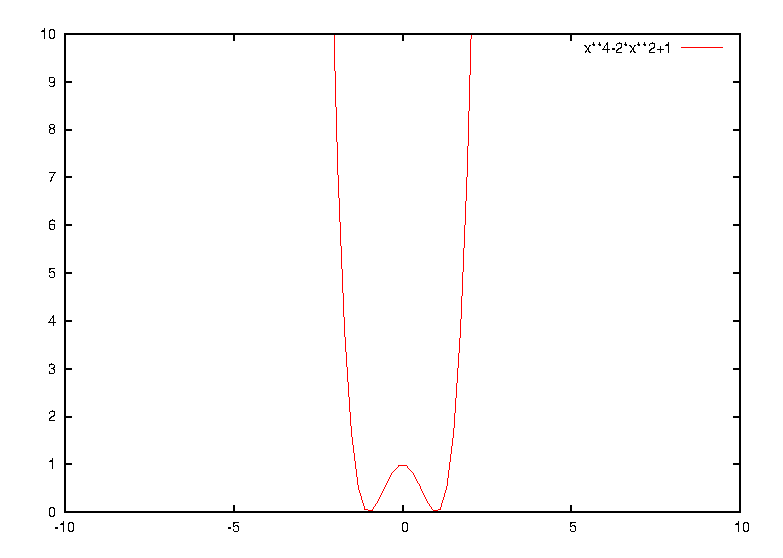
\includegraphics[width=5cm,bb=0 0 300 300]{14-1.eps}
\end{center}

%15
\section{}
\begin{flalign*}
	y=x\log{x}\\
	y'=\log{x}+1\ y'=0\text{を解くと} x=0,\pm1\\
		\begin{array}{c||c|c|c|c}\hline
		x	& 0 & \cdots &\frac{1}{e}  &\cdots \\\hline
		y'	&  \emTsya & -& 0 & +											\\\hline
		y	&  \emTsya &\searrow & 0 &\nearrow				\\\hline
	\end{array}
	\\\therefore x=\frac{1}{e}\text{のとき極小値}-\frac{1}{e},\text{極大値なし}
\end{flalign*}

%16
\section{}
\begin{flalign*}
	y=2\sin{x}-x\\
	y'=2\cos{x}-1 \ y'=0\text{を解くと} x=\frac{\pi}{3},\frac{5\pi}{3}\\
	\begin{array}{c||c|c|c|c|c|c|c}\hline
		x	& 0 & \cdots &\frac{\pi}{3} &\cdots & \frac{5\pi}{3} & \cdots & 2\pi														\\\hline
		y'	& 1 & + & 0 & - & 0 & + &1																																			\\\hline
		y	& 0 & \nearrow & \sqrt{3}-\frac{\pi}{3} &\searrow & -\sqrt{3}-\frac{5\pi}{3}	 & \nearrow & -2\pi		\\\hline
	\end{array}
	\\\therefore x=\frac{\pi}{3}\text{のとき最大値}\sqrt{3}-\frac{\pi}{3}\\
	x=\frac{5\pi}{3}\text{のとき最小値}-\sqrt{3}-\frac{5\pi}{3}
\end{flalign*}

%17
\section{}
\begin{flalign*}
	\text{(証明)}
	y=e^x-1-x \hspace{1cm} (x>0)\\
	y'=e^x-1 \hspace{1cm}y'=0\text{を解くと}x=0\\
	x>0\text{のとき}y>0\\
	\therefore y>0\\
	\therefore e^x>1+x\\
	Q.E.D.	
\end{flalign*}

%18
\section{}
\begin{flalign*}
	y=\frac{x^2+2x+2}{x+1}=x+1+\frac{1}{x+1}\\
	y'=1-\frac{1}{(x+1)^2}=\frac{x^2+2}{(x+1)^2}\\
	y'=0\text{を解くと}x=0,2,x\neq-1\\
	\begin{array}{c||c|c|c|c|c|c|c}\hline
		x	&  \cdots &-2 &\cdots & -1 & \cdots & 0	& \cdots	\\\hline
		y'	& + & 0 & - & \emTsya & - & 0 & +									\\\hline
		y & \NEE & -2 & \SES & \emTsya	 & \SEE & 2 & \NEN	\\\hline
	\end{array}
\end{flalign*}
\begin{center}
 	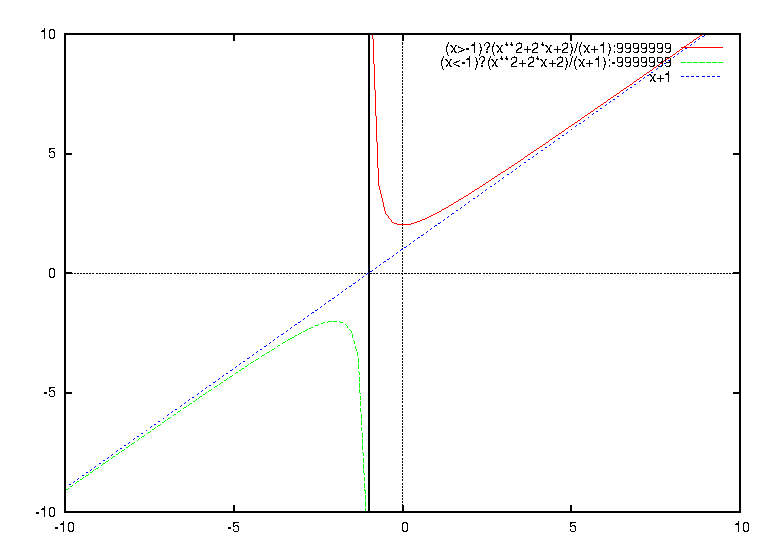
\includegraphics[width=5cm,bb=0 0 300 300]{18-1.eps}
\end{center}

%19
\section{}
\begin{enumerate}
\item \begin{flalign*}
	\int(3x+s)^4dx\\
	=\frac{1}{15}(3x+2)^5
\end{flalign*}
\item \begin{flalign*}
	\int \frac{1}{\sqrt[3]{x}}dx\\
	=\frac{3}{2}\sqrt[3]{x}^2
\end{flalign*}
\item \begin{flalign*}
	\int \frac{1}{2x-3}dx\\
	=\frac{1}{2}\log{|2x-3|}
\end{flalign*}
\item \begin{flalign*}
	\int \frac{1}{\cos^2{3x}}dx\\
	=\frac{1}{3}\tan{3x}
\end{flalign*}
\item \begin{flalign*}
	\int \frac{e^{4x}-e^x}{e^{2x}}dx\\
	=	\int (e^{2x}-e^{-x})dx\\
	=\frac{1}{2}e^{2x}+e^{-x}
\end{flalign*}
\item \begin{flalign*}
	\int \frac{1}{1+4x^2}dx\\
	=\frac{1}{2}\arctan{4x}
\end{flalign*}
\item \begin{flalign*}
	\int \frac{1}{\sqrt{2-x^2}}dx\\
	=\arcsin{\frac{x}{\sqrt{2}}}
\end{flalign*}
\item \begin{flalign*}
	&\int \frac{x^2-3}{x^2+3}dx\\
	&=\int 1-\frac{6}{x^2+3}\\
	&=x-2\sqrt{3}\arctan{\frac{x}{\sqrt{3}}}
\end{flalign*}
\item \begin{flalign*}
	\int \frac{x}{\sqrt{3+x}-\sqrt{3-x}}dx\\
	=\int \frac{x(\sqrt{3+x}+\sqrt{3-x})}{2x}dx\\
	=\frac{1}{2}\int(\sqrt{3+x}+\sqrt{3-x})dx\\
	=\frac{1}{3}(\sqrt{3+x}^3-\sqrt{3-x}^3)
\end{flalign*}
\item \begin{flalign*}
\end{flalign*}
\end{enumerate}

%13
\section{}
\begin{flalign*}
\end{flalign*}

%13
\section{}
\begin{flalign*}
\end{flalign*}

%13
\section{}
\begin{flalign*}
\end{flalign*}

%13
\section{}
\begin{flalign*}
\end{flalign*}

%13
\section{}
\begin{flalign*}
\end{flalign*}

\section{}
\begin{enumerate}
\item \begin{flalign*}
\end{flalign*}
\item \begin{flalign*}
\end{flalign*}
\item \begin{flalign*}
\end{flalign*}
\item \begin{flalign*}
\end{flalign*}
\item \begin{flalign*}
\end{flalign*}
\item \begin{flalign*}
\end{flalign*}
\item \begin{flalign*}
\end{flalign*}
\item \begin{flalign*}
\end{flalign*}
\end{enumerate}
\end{document}